\documentclass{standalone}
\usepackage[utf8]{vietnam}
\usepackage{amsmath,amsfonts,amssymb}
\usepackage{tikz}
\usetikzlibrary{patterns}
\begin{document}
	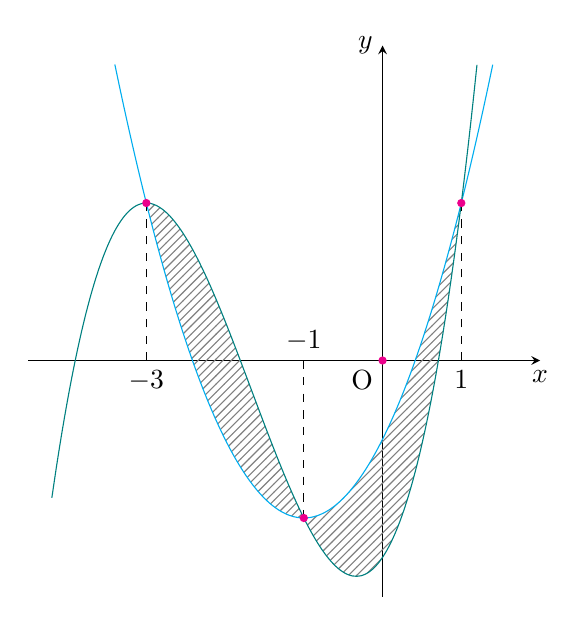
\begin{tikzpicture}[scale=1,>=stealth,smooth,samples=100]
		\def\f(#1){(#1)^2+2*(#1)-1}
		\def\g(#1){.5*(#1)^3+2.5*(#1)^2+1.5*(#1)-2.5}
		\draw[->] (-4.5,0)--(2,0) node [below]{$x$};
		\draw[->] (0,-3)--(0,4) node [left]{$y$};
		\fill[pattern=north east lines,pattern color=gray]
		plot[domain=-3:1] (\x,{\f(\x)})--
		plot[domain=1:-3] (\x,{\g(\x)})--cycle;
		\draw[cyan] plot[domain=-3.4:1.4] (\x,{\f(\x)});
		\draw[teal] plot[domain=-4.2:1.2] (\x,{\g(\x)});
		\draw[dashed]
		(0,0) node[below left]{O}
		(-3,0) node[below]{$-3$}--(-3,2)
		(-1,0) node[above]{$-1$}--(-1,-2)
		(1,0) node[below]{$1$}--(1,2);
		\foreach \p in {(0,0),(-3,2),(-1,-2),(1,2)}
		\fill[magenta] \p circle(1.5pt);
	\end{tikzpicture}
\end{document}